\documentclass[answers, 11pt]{exam}

\usepackage[spanish]{babel}
\usepackage[shortlabels]{enumitem}
\usepackage[T1]{fontenc}
\usepackage{graphicx}
\usepackage[cache=false,outputdir=./build]{minted}
\usepackage{lmodern}
\usepackage{wrapfig}
\usepackage{xcolor, color}
\definecolor{LightGray}{gray}{0.9}

\newcommand{\materia}{Analisis de Algoritmos 2024-1}
\newcommand{\tarea}{Tarea 07: Ordenamientos II}
\newcommand{\fecha}{\today}
\newcommand{\profesor}{Profesor(a): María de Luz Gasca Soto}
\newcommand{\ayudantes}{
  Rodrigo Fernando Velázquez Cruz \\
  Teresa Becerril Torres
}
\newcommand{\alumnos}{
  Alvaro Ramirez Lopez \textbf{N° cuenta:} 316276355
}

\decimalpoint{}
\graphicspath{{Imagenes}}
% \colorsolutionboxes
\shadedsolutions

% \definecolor{SolutionBoxColor}{rgb}{0,128,255}
% \definecolor{SolutionColor}{rgb}{0,204,255}
\definecolor{SolutionColor}{rgb}{0,128,255}

\renewcommand{\familydefault}{\sfdefault}

\extrawidth{1.56cm}
\extraheadheight[1.5in]{-0.25in}
\extrafootheight[-0.175in]{-0.375in}
\firstpageheader{
}{
  \begin{minipage}[c]{3.5cm}
    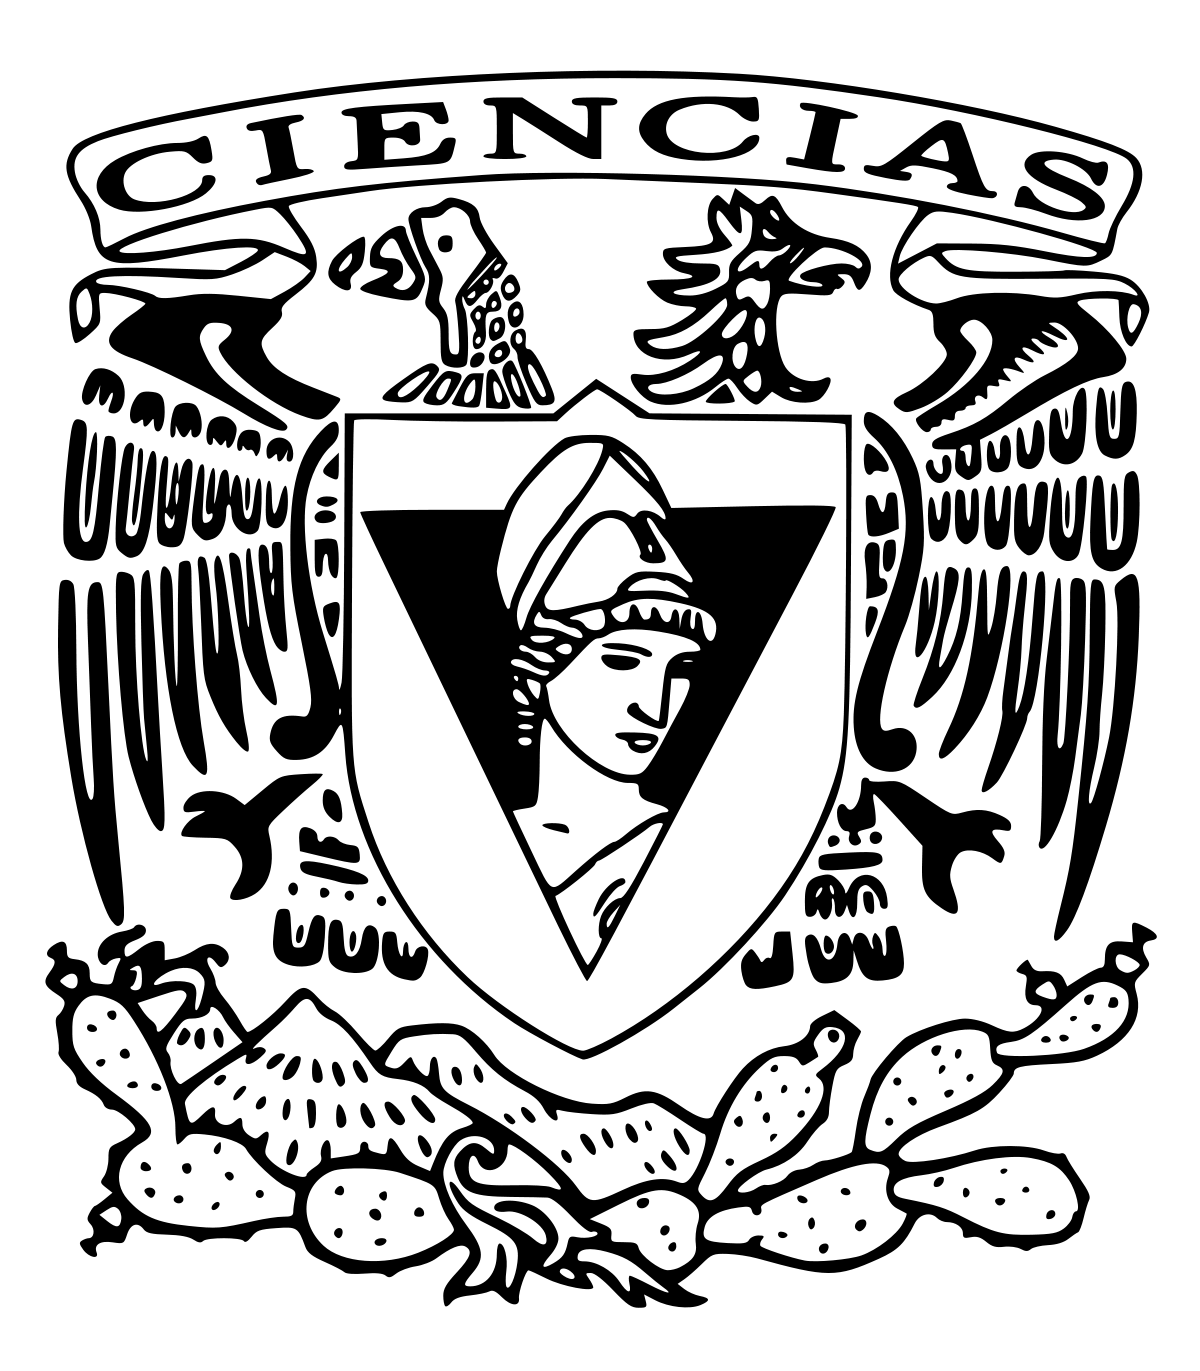
\includegraphics[width=3.5cm]{fc.png}
  \end{minipage}
  \begin{minipage}[c]{11.0cm}
    {\bfseries\huge\materia{} \\[2mm]
      \LARGE \tarea{} \\
      \large Profesor:} \profesor{} \\
    \hspace{0.1cm}
    {\bfseries\large Ayudantes:}
    \begin{minipage}[t]{8.5cm}
      \ayudantes{}\vspace{0.1cm}
    \end{minipage}\hfill\break{}
    {\bfseries\large Alumno:}
    \begin{minipage}[t]{8.5cm}
      \alumnos{}\\
    \end{minipage}\hfill\break{}
  \end{minipage}
  \begin{minipage}[c]{3.25cm}
    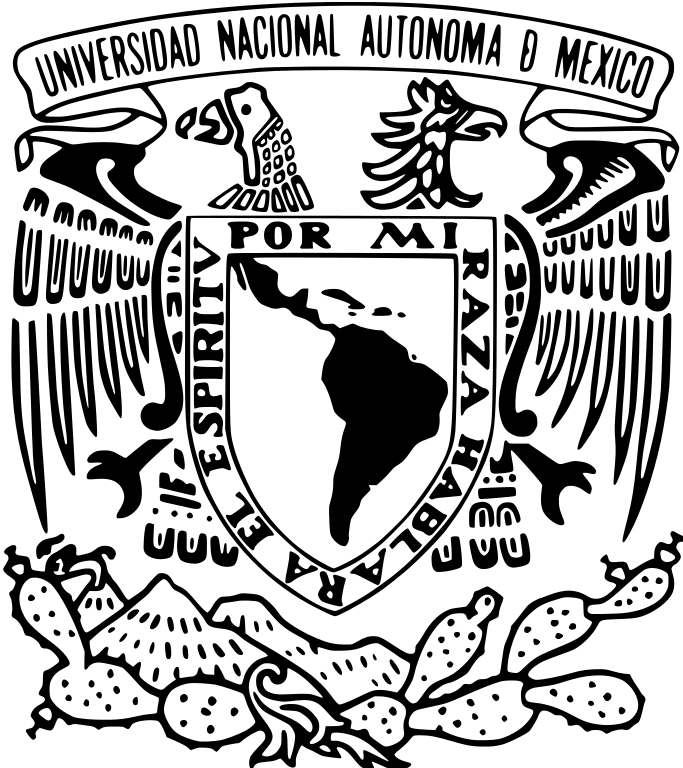
\includegraphics[width=3.25cm]{unam.png}
  \end{minipage}
}{}
\runningheader{\materia}{\tarea}{\fecha}
\runningheadrule{}
\footer{}{Página \thepage\ de \numpages}{}
\footrule{}
\renewcommand{\solutiontitle}{\noindent\textbf{Solución:}\par\noindent}



\begin{document}
\begin{questions}
\question{
El Problema de Seleccion consiste en encontrar el k-esimo elemento
mas pequeño de un conjunto de n datos. Utilizar las estrategias
usadas por el algoritmo \textbf{Quick Sort}, como el proceso Partition, para
resolver el problema de Selección. El algoritmo propuesto deberá tener
desempeño computacional de $O(n)$, en el caso promedio. Justifique
con detalle sus respuestas.
}

\begin{solution}
  Aqui va la respuesta
\end{solution}

\question{
Sea \textbf{QuickSort 1} la versión de \textit{Quick Sort} que toma como pivote al
elemento $A[(first + last) \verb| div | 2]$; y sea Sea \textbf{QuickSort 2} la versión que
toma como pivote al elemento que resulta ser la mediana de $A[first]$, 
$A[(first + last) \verb| div | 2]$, $A[last]$.

Dar un ejemplo de una lista de al menos 23 valores donde el desempeño
computacional de \textbf{QuickSort 2} sea mejor que el de \textbf{QuickSort 1}
}

\begin{solution}
  Aqui va la respuesta
\end{solution}

\question{
Proporcione una secuencia $L$ de enteros diferentes, de tres dígitos cada
uno. Considere $|L| \geq 30$
Aplique \textbf{Bucket Sort} a $L$ de dos maneras distintas.
}

\begin{solution}
  Aqui va la respuesta
\end{solution}

\question{
Proporcione una secuencia $L$ de enteros diferentes, en hexadecimal, de
cuatro cifras cada uno. Considere $|L| \geq 25$
\begin{enumerate}[a)]
  \item Ordena la secuencia usando...
  \begin{enumerate}[i)]
    \item ... MSD-Radix-Sort;
    \item ... LSD-Radix-Sort;
  \end{enumerate}
  \item Comente sobre las ejecuciones
\end{enumerate}
}

\begin{solution}
  Aqui va la respuesta
\end{solution}

\question{
\textbf{Opcional} Sea $L$ una lista de $n$ numeros enteros diferentes. Suponga
que los elementos $x$ de $L$ están en el intervalo $[1, 500]$.
Diseñe un algoritmo de orden lineal que ordene los elementos de $L$.
}

\begin{solution}
  Aqui va la respuesta
\end{solution}
  
\end{questions}
\end{document}

